\chapter{Water Tank (Periodic)} \label{chap:watertankperiodic}
\section{Case Description}
This model is an implementation of a water tank that is supplied by a
flow of water.  There is a valve at the bottom of the tank which can
be opened so that water flows out of the tank, or closed to stop the
exiting flow of water.  Underneath the tank we assume that there is a
drain to catch the outflowing water.  The tank is equipped with a
sensor to measure the current water level.

Figure \ref{fig:waterTank} illustrates the tank, the water flowing in,
the valve and the drain as components in a CT model, with a DE model
providing a controller.

\begin{figure}[!ht]
\centering
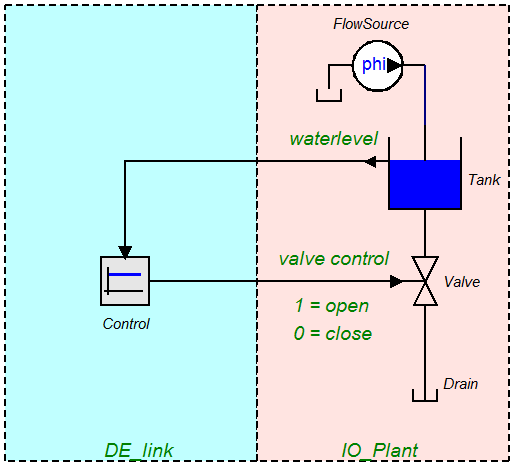
\includegraphics[width=7cm]{waterTankPeriodic/WaterTank.png}
\caption{Overview of the water tank in the case
  study \label{fig:waterTank}}
\end{figure}

We should like the water in the tank to remain between some maximum
and some minimum level.  If the water level falls below our minimum
desired level then the valve must be closed to ensure water stops
flowing out of the tank.  If the water rises above our maximum desired
level, then the valve must be opened to enable water to flow out.
This particular water tank model accomplishes this by polling the
water level sensor periodically, at intervals of \emph{n}
milliseconds, to monitor the current water level, checking that it
falls within acceptable boundaries, and taking some action if it does
not.

\section{Contract}
The contract for the periodic water tank model includes one
\emph{monitored} variable of type \keyw{real} (called \texttt{level})
which represents the current level of water measured by the sensor.
And there is one \emph{controlled} variable of type \keyw{bool}
(called \texttt{valve}) which is a signal to open or shut the valve.

In addition, there are two shared design parameters of type
\keyw{real}: \texttt{maxlevel} and \texttt{minlevel}, which dictate
the desired maximum and minimum level of the water respectively.  The
shared design parameters can be configured at runtime when executing a
simulation of the model, by opening the debug configuration options in
the \DESTECS tool before the simulation is started.

\section{Discrete-event}
The DE model contains a \texttt{Controller} class, which has the main
thread of control.  An instance of \texttt{LevelSensor} is created to
represent the sensor that measures the current water level.  An
instance of \texttt{ValveActuator} is created to represent the valve
at the bottom of the tank.  \texttt{LevelSensor} simply returns a
value to represent the current level of water, whilst
\texttt{Valve\-Ac\-tu\-a\-tor} accepts a boolean value that sets the valve to
be open or closed.

The \texttt{Controller} starts a single thread that loops repeatedly,
waiting for some milliseconds \emph{n} and then collecting a reading
from the water level sensor.  If the level is calculated to be above
the desired maximum level then \texttt{Controller} sets the valve to
be open, calling the appropriate method in the \texttt{ValveActuator}
class.  Similarly, if the water level is calculated to be below the
desired minimum level then \texttt{Controller} sets the valve to be
closed.  The same thread continues to loop.

The \texttt{Controller} is deployed onto a single CPU
by the \texttt{System} class.

\section{Continuous-time}
The CT model for the periodic water tank consists of two main parts,
one to represent the link to the DE side of the model (\texttt{DE\_link})
and one to represent the CT side (\texttt{I\_O\_Plant}).

The \texttt{DE\_link} block handles interaction with the DE
model itself.  It contains a block, \texttt{Control}, which handles
the input from the DE model (\texttt{valve}, to represent a signal for
the valve actuator) and also the output from the CT model
(\texttt{level}, which represents the current water level as read by
the sensor).  These are the shared variables declared in the contract.

The \texttt{I\_O\_Plant} block incorporates other blocks to
represent the plant.  There is a \texttt{Flow\-Sour\-ce} to represent the
source of incoming water, a \texttt{tank} to contain the water and a
\texttt{Valve} at the bottom of the tank to control outward flow.
Underneath the tank is a \texttt{Drain}.

\section{Usage}
Running a simulation of the periodic water tank illustrates how
the water level in the tank rises until the maximum level is reached,
at which point the valve is opened and the level falls until the
minimum is reached.  The valve is then closed again and the process
repeats itself.  One way to experiment with the model is to change the
shared design parameters which dictate the values for the maximum and
minimum water levels.  These can be set in the Debug configuration
window in the \DESTECS tool.  We recommend changing the values and
running the co-simulation with these varying values to view the effect
on the behaviour of the system.
